
\documentclass{beamer}
%
% LVM Seminar
% Copyright 2018, Aswin Babu Karuvally
%
\mode<presentation>
{
    \usetheme{default}
    \usecolortheme{beaver}
    \usefonttheme{default}
    \setbeamertemplate{navigation symbols}{}
    \setbeamertemplate{caption}[numbered]
} 

\usepackage[english]{babel}
\usepackage[utf8x]{inputenc}

\title[Your Short Title]{Comparison and Performance Analysis of Standard and
LVM Based Disk Partitioning}
\author{Aswin Babu K}
\institute{College of Engineering Trivandrum}
\date{16th September 2018}

\begin{document}

\begin{frame}
    \titlepage
\end{frame}

\begin{frame}{File Systems}
    \begin{itemize}
        \item<2-> Computers use secondary storage for permanent data storage
        \item<3-> File Systems specify the format for read/write tasks
        \item<4-> Examples: ext4, XFS, FAT32, NTFS
        \item<5-> Partitions are containers on which file systems are created
        \item<6-> Partitions need not be the entire size of the drive
        \item<7-> Creating multiple partitions is the norm
        \item<8-> Each partition need not have the same file system
    \end{itemize}
\end{frame}

\begin{frame}{Disk Partitioning}
    \begin{itemize}
        \item<2-> The process of creating partitions
        \item<3-> Entirely logical process
        \item<4-> Partition utilities include fdisk, parted and diskutil
    \end{itemize}
\end{frame}

\begin{frame}{Why multiple Partitions?}
    \begin{itemize}
        \item<2-> Separate user data from system files
        \item<3-> Run multiple Operating Systems
        \item<4-> Organize personal data
    \end{itemize}
\end{frame}

\begin{frame}{Partition Table}
    \begin{itemize}
        \item<2-> Stores information about the partitions
        \item<3-> Several formats exist, eg. APM, MBR, GUID, diskLabel
        \item<4-> Most of the older PCs use Master Boot Record
        \item<5-> Newer PCs use GUID Partition Table
    \end{itemize}
\end{frame}

\begin{frame}{Partition Table}
    \begin{figure}
        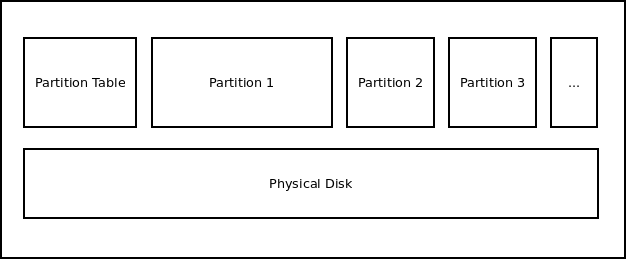
\includegraphics[scale=0.45]{partitions.png}
        \caption{A typical partition table}
    \end{figure}
\end{frame}

\begin{frame}{Disadvantages of Standard Partition Model}
    \begin{itemize}
        \item<2-> Mounted partitions cannot be manipulated 
        \item<3-> Partitions can use only adjacent free space during resize
        \item<4-> You cannot extend a partition to cover two physical drives
    \end{itemize}
\end{frame}

\begin{frame}{Logical Volume Manager}
    \begin{itemize}
        \item<2-> An abstraction on top of an abstraction
        \item<3-> Creates logical volumes, on top of existing partitions
        \item<4-> Existing partitions are called Physical Volumes (PV)
        \item<5-> One or more physical volumes form Volume Groups (VG)
        \item<6-> Logical Volumes (LV) are created on top of VGs
        \item<7-> Device Mapper acts as middle man between LVM and Linux
    \end{itemize}
\end{frame}

\begin{frame}{Logical Volume Manager}
    \begin{figure}
        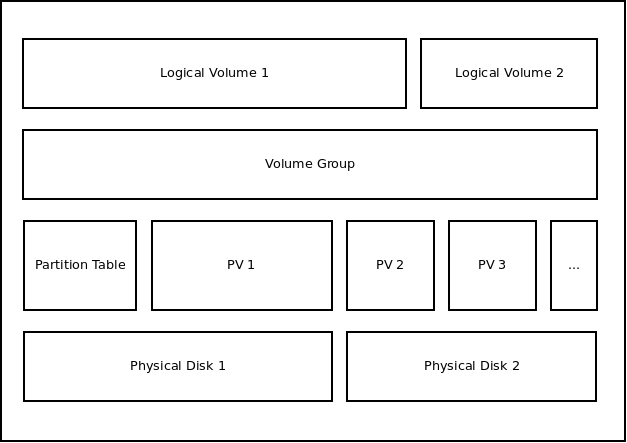
\includegraphics[scale=0.4]{lvm.png}
        \caption{A typical LVM setup}
    \end{figure}
\end{frame}

\begin{frame}{Advantages of LVM}
    \begin{itemize}
        \item<2-> Mounted volumes can be manipulated
        \item<3-> Partitions can span more than one physical drive
        \item<4-> Creation of snapshots while system is up
        \item<5-> Allows creating striped volume
    \end{itemize}
\end{frame}

\begin{frame}{Source Code} 
    \begin{center}
        \large https://github.com/karuvally/project\_green.git
    \end{center}
\end{frame}

\end{document}
